%%%%%%%%%%%%%%%%%%%%%%%%%%%%%%%%%%%%%%%%%%%%%%%%%%%%%%%%%%%%%%%%%%%%%%%%%%%%%%%
%% LaTeX-Vorlage für Abschlussarbeiten (Koma-Script)                         %%
%% (TH Köln -Campus Gummersbach, Fak. 10)                                    %%
%%                                                                           %%
%% Gemäß dem Merkblatt zur Anfertigung von Projekt-, Bachelor-, Master- und  %%
%% Diplomarbeiten der Fakultät 10 von Frau Prof. Dr. Halfmann &              %%
%% Herr Prof. Dr. Rühmann (Version vom 27.01.2008)                           %%
%%                                                                           %%
%% LIZENZ:                                                                   %%
%% Diese Vorlage darf nicht kommerziell verbreitet                           %%
%% werden. Eine nicht-kommerzielle Weitergabe ist                            %%
%% gestattet.                                                                %%
%%                                                                           %%
%% Von Ludger Schönfeld, M. Sc.,                                             %%
%% 2015-2017 (Stand: 05.04.17)                                               %%
%%%%%%%%%%%%%%%%%%%%%%%%%%%%%%%%%%%%%%%%%%%%%%%%%%%%%%%%%%%%%%%%%%%%%%%%%%%%%%%

\documentclass[a4paper,fontsize=12pt,abstract=true, toc=nolistof,headsepline=true,footsepline=true]{scrartcl}
%%INFO: Dokumenteinstellungen
% - fontsize: Schriftgröße (hier jede beliebige, Standard: 11pt)
% - abstract: Überschrift zum Abstract ein-/abschalten (Werte: true/false)
% - toc: Gestalt des Inhaltsverzeichnisses beeinflussen (s. KOMA-Script-Guide).
%   Wert "listof/nolistof" => Verzeichnisse von Tabellen & Abbildungen werden unnummeriert ins Inhaltsverzeichnis aufgenommen bzw. nicht ins Inhaltsverzeichnis aufgenommen.
% - headsepline: Ein-/Ausschalten einer Linie in der Kopfzeile.
% - footsepline: Ein-/Ausschalten einer Linie in der Fusszeile.
%

\usepackage[ngerman]{babel}
\usepackage[T1]{fontenc} % Schriftkodierung (Für Sonderzeichen u.a.)
\usepackage[utf8]{inputenc} % Für die direkte Eingabe von Umlauten im Editor u.a. - ACHTUNG: Kodierung muss mit der Zeichenkodierung im Editor übereinstimmen!
\usepackage{microtype} % Verbesserter Randausgleich
\usepackage{lmodern}
\usepackage{parskip}

%% Paket für Beispiel-Text (Pseudo-Latein)
% => Befehl (Bsp.): \lipsum[2-4]
\usepackage{lipsum}

%% Zeilenabstand setzen
\usepackage[onehalfspacing]{setspace}
% INFO: Zeilenabstand setzen:
%
% Befehle:
% - \singlespacing  => 1-zeilig (Standard)
% - \onehalfspacing => 1,5-zeilig
% - \doublespacing  => 2-zeilig

%% Satzspiegel einrichten
\usepackage[left=3cm,right=2cm,top=1.5cm,bottom=1cm,
    textheight=245mm,textwidth=160mm,includeheadfoot,headsep=1cm,
    footskip=1cm,headheight=14.599pt]{geometry} % Einrichtung der Seite
% KOMA-Script bietet das Paket "typearea". Dieses berechnet Ihnen eine optimale Seiteneinstellung. Bei diesem Paket haben Sie allerdings nicht so viele Einstellungsmöglichkeiten.

%% Einstellungen für Marginalien (Beispiel)
%%(Randkommentierung mit \marginpar{Text})
%\newcommand\mpar[1]{\marginpar {\flushleft\sffamily\small #1}}
%\setlength{\marginparwidth}{3cm}

%% Einbinden von Graphiken
\usepackage{graphicx}
\usepackage{epstopdf} % Umwandlung EPS-Bilder => PDF, sodass diese auch mithilfe des Tools "pdflatex" eingebunden werden können
% Unterstreichen von Text
\usepackage[normalem]{ulem} % Befehl: \uline{}

%% Pakete für Tabellen
\usepackage{tabularx} % Einfache Tabellen
\usepackage{longtable} % Tabellen als Gleitobjekte (für die Aufteilung bei langen Tabellen über mehrere Seiten)
\usepackage{multirow} % Verbinden von Zeilen innerhalb einer Tabelle mit \multirow{anzahl}{*}{Text}
\usepackage{pbox}

% (Zusatz-)Pakete für Formeln
\usepackage{amsmath}
\usepackage{amsthm}
\usepackage{amsfonts}

% Farbboxen (für die Merkkästen in dieser Vorlage):
\usepackage{tcolorbox}
\tcbset{colback=white,colframe=orange,
    fonttitle=\bfseries}

%% Autom. Literaturverzeichnisse mit dem Paket 'biblatex'":
\usepackage{biblatex}
\addbibresource{bib/sources.bib}

\usepackage[colorlinks,pdfpagelabels,pdfstartview=FitH,
    bookmarksopen=true,bookmarksnumbered=true,linkcolor=black,
    plainpages=false,hypertexnames=false,citecolor=black]{hyperref} % Für Verlinkungen
% INFO: Verlinkungen mit dem hyperref-Paket:
%
% Die Angabe von URLs mit dem Befehl \url{} erlaubt einen
% gesonderten Umgang mit Weblinks. Denn die Links werden verlinkt.
% Auch erfolgt automatisch am Zeilenende ein Umbruch des Links.
% Es ist auch nicht erforderlich, Sonderzeichen in der URL manuell zu
% entschärfen.
%
% TIPP: Sollte ein Umbruch bei einem Link nicht automatisch erfolgen, so kann
% das daran liegen, dass ein/mehrere Zeichen zusätzlich angegeben werden müssen,
% an dem der Link umbrochen werden kann.
% => Siehe Paket "breakurl"

\usepackage{pdfpages}

\usepackage{color}
\usepackage{xcolor}

\usepackage{array,etoolbox}
\usepackage{csquotes}
\preto\tabular{\setcounter{magicrownumbers}{0}}
\newcounter{magicrownumbers}
\newcommand\rownumber{\stepcounter{magicrownumbers}\arabic{magicrownumbers}}

\newcommand{\newlineparagraph}[1]{\paragraph{#1}\mbox{}\\}

\begin{document}
    \pagestyle{empty}
\begin{titlepage}
    
\includegraphics[scale=1.0]{assets/logo_TH-Koeln_CMYK_22pt}\\
    \begin{center}
        \large
        Technische Hochschule Köln\\
        Fakultät für Informatik und Ingenieurwissenschaften\\
        \vspace{1cm}
        \large
        \textsc{Bachelorarbeit}\\
        \vspace{1cm}
        \huge
        Vergleichende Analyse von\\
        Laravel Admin-Panels mittels\\
        Software Design Principles und Patterns\\
        sowie prototypischer Implementierung\\
        \vspace{1cm}
        \large
        vorgelegt an der TH Köln\\
        Campus Gummersbach\\
        im Studiengang\\
        Medieninformatik\\
        \vspace{1cm}
        ausgearbeitet von:\\
        \textsc{Niklas Canisius}\\
        (Matrikelnummer: 11110023)\\
        \vspace{1cm}
        \begin{tabular}{ll}
            \textbf{Erster Prüfer:} & Prof.\ Dr. Christian Kohls \\
            \textbf{Zweiter Prüfer:} & Johannes Frielingsdorf \\
        \end{tabular}
        \vspace{1cm}
        \\Gummersbach, den \today
    \end{center}
\end{titlepage}

    \newpage


\section*{Sperrvermerk}
Das vorliegende Dokument beinhaltet vertrauliche Daten der Firma Graw Radiosondes GmbH \& Co. KG.
Es darf nur von berechtigten Personen innerhalb ihrer dienstlichen Verpflichtungen eingesehen werden.

Eine Veröffentlichung und Vervielfältigung – auch in Teilen – ist nicht gestattet.
Dritten darf dieses Dokument nur mit der ausdrücklichen Genehmigung des Verfassers und des Unternehmens zugänglich gemacht werden.

Der Sperrvermerk gilt für ein Jahr ab dem \today.

    \newpage


\section*{Abstract}


    \newpage
    \renewcommand{\contentsname}{Inhaltsverzeichnis}
    \tableofcontents
    \newpage

    \pagestyle{headings} % Kopf- und Fußzeilen aktivieren
    \pagenumbering{arabic} % Seitennummerierung: arabische Zahlen

    \section{Einleitung}

Diese Arbeit baut auf der vorangegangenen Praxisprojektarbeit auf.
Diese trägt den Titel \enquote{Praktische Evaluation des Frameworks Laravel Nova am Beispiel einer Anwendung zur Verwaltung und Auswertung von Radiosondenaufstiegen}.
In dieser Arbeit zeigten sich Probleme mit Nova, vor allem in puncto Anpassbarkeit.
Ebenfalls wurden in einer Nutzwertanalyse geeignete Alternativen zu Nova identifiziert.
Dabei wurde vor allem das Framework filament~\cite{filament} als bessere Alternative herausgearbeitet.
Unter Betrachtung dieser kurzen Vorstudie entsteht die Bachelorarbeit.
Die beiden Frameworks Nova und filament sollen anhand von Software Design Principles und Patterns, sowie prototypischer Implementierung, verglichen werden.

\subsection{Fragestellung}
Im Rahmen dieser Arbeit soll die Frage geklärt werden, ob für das vorliegende Projekt der \enquote{Sounding Console} Nova oder filament besser geeignet ist.

\subsection{Zielsetzung}
Ziel dieser Arbeit ist zum einen die prototypische Umsetzung einiger Features der Sounding Console mittels filament.
Dabei sollen praktische Erfahrungen mit dem Framework gesammelt werden um diese mit den bei Nova vorhandenen Erfahrungen zu vergleichen.

Zum anderen soll ein theoretischer Vergleich der beiden Frameworks durchgeführt werden.

Als finales Ergebnis soll die Fragestellung bewertet werden und damit der weitere Weg für die Applikation bestimmt werden.

    \section{Grundlagen}
Die theoretische Basis für den Vergleich bieten verschiedene Software Design Principles und Patterns, welche
im Folgenden eingeführt werden.

\subsection{Principles}
Software Design Principles sind weder Regeln, Gesetze noch perfekte Wahrheiten.
Stattdessen sind diese Prinzipien Empfehlungen bzw.\ Ratschläge.
(Vgl.~\cite{getting-a-solid-start})

Software Design Prinzipien sind Heuristiken und allgemeingültige Lösungen für übliche Probleme.
Sie wurden empirisch beobachtet und gelten daher meistens, allerdings auch nicht unbedingt immer.
(Vgl.~\cite{getting-a-solid-start})

https://www.geeksforgeeks.org/principles-of-software-design/

https://www.dotnettricks.com/learn/designpatterns/different-types-of-software-design-principles

\subsubsection{SOLID Principles}
Die Kerngruppe der Software Design Prinzipien werden von Robert C. Martin unter dem Titel \enquote{The Principles of OOD}(\cite{solid}) beschrieben.
Die Grundlage dafür legte er in seinem Paper \enquote{Design Principles and Design Patterns}(\cite{design-principles-and-design-patterns}) im Jahr 2000.

https://medium.com/successivetech/s-o-l-i-d-the-first-5-principles-of-object-oriented-design-with-php-b6d2742c90d7

https://www.digitalocean.com/community/conceptual-articles/s-o-l-i-d-the-first-five-principles-of-object-oriented-design#interface-segregation-principle

https://accesto.com/blog/solid-php-solid-principles-in-php/

\paragraph{Single Responsibility Principle}
\enquote{A class should have one, and only one, reason to change.}(\cite{solid})

\paragraph{Open Closed Principle}
\enquote{You should be able to extend a classes' behavior, without modifying it.}(\cite{solid})

\paragraph{Liskov Substitution Principle}
\enquote{Derived classes must be substitutable for their base classes.}(\cite{solid})

\paragraph{Interface Segregation Principle}
\enquote{Make fine-grained interfaces that are client specific.}(\cite{solid})

\paragraph{Dependency Inversion Principle}
\enquote{Depend on abstractions, not on concretions.}(\cite{solid})

\subsubsection{Boy Scout Rule}
Sinnvoll im Projektkontext?
\subsubsection{PSR (PHP Standards Recommendations)}
The PHP Framework Interop Group is working on and publishes PSRs (PHP Standards Recommendations).(Vgl. \cite{psr})

\subsubsection{KISS (Keep It Simple Stupid)}
\begin{itemize}
    \item Don't complicate the code.
    \item The code should be its documentation itself.
    \item Any new programmer on the team should be able to get into the project quickly.
\end{itemize}
\subsubsection{DRY (Don’t Repeat Yourself)}
Do not code using the Copy-Paste principle (there is no such rule).

See that the same code repeats in several places? Extract code for a separate function.
\subsubsection{YAGNI (You Aren’t Gonna Need It)}
We should not write code “for the future”.

Such code is not needed at the moment.
\subsubsection{GRASP (General Responsibility Assignment Software Patterns)}
GRASP is a large set of rules about which I could write a separate article.
These are the basic principles that we should follow when creating object design and responsibility assignments.
It consists of: Information Expert, Controller, Creator, High Cohesion, Low Coupling, Pure Fabrication, Polymorphism, Protected Variations, Indirection.

\subsection{Patterns}
Patterns, sogenannte Entwurfsmuster, wurden ursprünglich vom Architekten Christopher Alexander geprägt.
Dieser beschrieb in seinem Buch \enquote{A Pattern Language: Towns, Buildings, Construction}(\cite{a-pattern-language}) im Jahr 1977 zum ersten Mal Muster, unter dessen Einsatz man immer wiederkehrende Probleme lösen kann.
In der Informatik wurden Entwurfsmuster durch die Veröffentlichung der \enquote{Gang of Four} im Jahr 1994 populärer.
In ihrem Buch \enquote{Design Patterns - Elements of Reusable Object-Oriented Software}(\cite{gamma-design-patterns}) beschreiben Erich Gamma et al.\ 23 unterschiedliche Entwurfsmuster.
Diese sind eingeteilt in die drei Kategorien Creational, Structural und Behavioral.

1999 ergänzte Martin Fowler in \enquote{Patterns of Enterprise Application Architecture}(\cite{patterns-of-enterprise-application-architecture}) die Kategorie \enquote{Objektrelationale Abbildung} und dazugehörige Muster.
Gregor Hohpe und Bobby Woolf ergänzten 2003 die Kategorie der Messaging Patterns in ihrem Buch \enquote{Enterprise Integration Patterns}(\cite{enterprise-integration-patterns}).

Die Menge der Entwurfsmuster ist so umfangreich, dass eine wiedergabe aller an dieser Stelle weder von Nutzen noch machbar wäre.
Im Folgenden werden daher nur die Muster eingeführt, die im anschließenden Vergleich verwendet werden.

    \section{Analyse}
Die Basis für den praktischen Teil dieser Arbeit ist die auf Basis von Laravel und Nova bereits entwickelte Sounding Console.
Um den Funktionsrahmen für den Prototypen zu definieren, müssen die Probleme mit dem bestehenden MVP (Minimal Viable Product) identifiziert werden.

Die Basis für den theoretischen Teil liefern anerkannte Software Design Principles und Patterns.
Es wird geklärt, welche Principles und Patterns im vorliegenden technischen Anwendungskontext grundsätzlich zur Anwendung kommen können.

Zusätzlich bietet der jeweilige Funktionsumfang der Frameworks eine sinnvolle Vergleichsbasis.
Dafür wird eine geeignete Vergleichsmethodik identifiziert, definiert und durchgeführt.

Weitere mögliche Vergleichsaspekte sind die Maturity der beiden Frameworks, der verwendete Code Style, ein Kostenvergleich und Unterschiede in der Lizenzierung.
Es wird erarbeitet, inwiefern diese Aspekte vergleichbar sind.

\subsection{Probleme des bisherigen Prototyps}
Im Rahmen der Nutzwertanalyse wurde vermutet, dass filament anpassbarer als Nova ist.
Insbesondere die Flight View wurde in Tests mit Anwendern kritisiert.
Nova ist recht eingeschränkt in der Platzierung von individuellen Komponenten innerhalb einer View.
Im praktischen Prototyp soll geprüft werden, ob filament in diesem konkreten Fall besser angepasst werden kann.
Des Weiteren ergaben sich die folgenden Probleme bei der Umsetzung des MVP mit Nova.

\newlineparagraph{Styling von Custom Components}
Trotz individueller Komponenten wird ein einheitliche UI (User Interface) angestrebt.
Dazu werden innerhalb der individuellen Komponenten UI-Components von Nova importiert.
Dies ist bei Nova allerdings nicht vorgesehen, es wird geklärt, ob sich dies bei filament anders darstellt.

\newlineparagraph{Infinite Loading Tables}
Die unschön gelösten Infinite Loading Tabellen in Nova, sind problematisch, da die Funktion mit einem Update jederzeit unbrauchbar gemacht werden könnte.
Filament bietet in der Pagination die Möglichkeit, alle Datensätze in einer Tabelle zu laden.
Es wird daher geprüft, ob die Performance ausreichend ist oder ob es eine andere Lösung gibt.

\newpage

\newlineparagraph{Tabellensortierung}
Die fehlende Möglichkeit, bei der Messwertetabelle eine Standardsortierung zu definieren, ist nach wie vor ein Problem.
Beim Einsatz von filament wird geprüft, ob dieses Problem gelöst werden kann.

\newlineparagraph{Polling Tables}
Manche Tabellen, beispielsweise die Stationsübersicht, sollen in einem gewissen Interval automatisch abgerufen werden.
Dadurch soll der Anwender stets erkennen können, welche Stationen aktuell online sind und welche nicht.
Nova bietet diese Funktionalität, allerdings ist die Animation sehr störend.
Die Tabelle verschwindet für einen Moment und dadurch ist ein einfacher Vergleich eher schwierig.
Außerdem wird die Tabelle kürzer und dadurch springt die ganze Seite.

Filament bietet das notwendige Feature ebenfalls.
Es wird im Prototyp daher geprüft, ob die Animation besser umgesetzt ist.

\subsection{Geeignete Principles und Patterns}
\begin{itemize}
    \item welche Principles sind geeignet
    \item welche Patterns sind geeignet
    \item Diskussion alternativer Vorgehensweisen
\end{itemize}

tbd

\newpage
\section{Konzeption}

\subsection{Anforderungen an den neuen Prototyp}
\color{red}
Vergleichbar mit den Anforderungen als Tabelle im PP.

tbd
\color{black}

\subsection{Vergleichsmethodik: Funktionsumfang}
\color{red}
Die bereits durchgeführte Methodik definieren.

tbd
\color{black}

\subsection{Vergleichsmethodik: Principles und Patterns}
\color{red}
Wie werden die passenden Principles und Patterns verglichen?

tbd
\color{black}


    \addtocontents{toc}{\protect\newpage}

\section{Durchführung}

\subsection{Vergleich auf Basis der Features}
\begin{table}[]
    \caption{Featurevergleich}
    \label{tab:feature-comparison}
    \resizebox{\textwidth}{12.2cm}{%
        \begin{tabular}{llclcl}
            \textbf{Category}                        & \textbf{Feature}       & \textbf{10} & \textbf{Nova}                   & \textbf{34} & \textbf{Filament}                        \\
            \hline
            \multirow{2}{*}{\textbf{Technical}}      & Laravel Support        & n           & \textgreater{}= 8.0             & n           & \textgreater{}= 8.0                      \\
            & PHP Support            & g           & \textgreater{}= 7.3             & n           & \textgreater{}= 8.0                      \\
            \hline
            \multirow{10}{*}{\textbf{Resources}}     & Number of fields       & g           & 38                              & b           & 16                                       \\
            & Computed fields        & g           & yes                             & g           & yes                                      \\
            & Repeater fields        & b           & no                              & g           & supported                                \\
            & Builder fields         & b           & no                              & g           & supported                                \\
            & Table polling          & n           & yes, but bad animation          & g           & yes                                      \\
            & Filters                & g           & supported                       & g           & supported                                \\
            & Lenses                 & g           & supported                       & b           & no                                       \\
            & Actions                & n           & title, fields \& responses      & g           & title, fields, responses \& custom views \\
            & Queued Actions         & g           & supported                       & n           & only custom                              \\
            & Action log             & g           & supported                       & b           & no                                       \\
            \hline
            \multirow{3}{*}{\textbf{Custom views}}   & Custom pages/Tools     & n           & complicated but powerful        & g           & simple and powerful                      \\
            & Custom resource pages  & b           & no                              & g           & yes                                      \\
            & Widgets/Cards          & n           & complicated but powerful        & g           & simple and powerful                      \\
            \hline
            \multirow{12}{*}{\textbf{Search}}        & Searchable Columns     & g           & can be defined                  & g           & can be defined                           \\
            & Title                  & g           & can be defined                  & g           & can be defined                           \\
            & Details/Subtitle       & g           & can be defined                  & g           & can be defined                           \\
            & Url                    & b           & no                              & g           & can be defined                           \\
            & Actions                & b           & no                              & g           & can be defined                           \\
            & Full-Text Indexes      & g           & supported                       & b           & no                                       \\
            & Searching Relations    & g           & supported                       & b           & not clear, probably not supported        \\
            & Searching JSON Data    & g           & supported                       & b           & not clear, probably not supported        \\
            & Limits                 & g           & supported                       & b           & no                                       \\
            & Debounce timing        & g           & supported                       & b           & no                                       \\
            & Global disable         & g           & supported                       & b           & no                                       \\
            & Laravel Scout          & g           & supported                       & n           & can be customized                        \\
            \hline
            \multirow{15}{*}{\textbf{Metrics}}       & Value                  & g           & avg/sum/max/min                 & n           & yes, but no predefined functions         \\
            & Trend/Line             & g           & count/avg/sum/max/min           & n           & yes, but no predefined functions         \\
            & Bar                    & b           & no                              & g           & yes                                      \\
            & Bubble                 & b           & no                              & g           & yes                                      \\
            & Polar Area             & b           & no                              & g           & yes                                      \\
            & Radar                  & b           & no                              & g           & yes                                      \\
            & Scatter                & b           & no                              & g           & yes                                      \\
            & Partition/Pie/Doughnut & g           & avg/sum/max/min                 & n           & yes, but no predefined functions         \\
            & Progress               & g           & count/sum                       & b           & no                                       \\
            & Custom chart control   & b           & no                              & g           & yes, configure the chart.js options      \\
            & Table                  & n           & icon, title, subtitle \& action & g           & multiple columns, filters \& actions     \\
            & Ranges                 & g           & can be defined                  & g           & can be defined                           \\
            & Caching                & g           & supported                       & b           & no                                       \\
            & Formatting             & n           & possible but limited            & g           & possible                                 \\
            & Polling                & n           & some events                     & g           & interval                                 \\
            \hline
            \multirow{3}{*}{\textbf{Dashboard}}      & widget width           & n           & yes                             & g           & yes, responsive                          \\
            & grid col number        & b           & no                              & g           & yes, responsive                          \\
            & conditionally hiding   & g           & yes                             & g           & yes                                      \\
            \hline
            \multirow{5}{*}{\textbf{Notifications}}  & Content                & n           & title, action, icon \& type     & g           & title, body, action, icon \& type        \\
            & Global disable         & g           & supported                       & b           & no                                       \\
            & Duration               & b           & no                              & g           & supported                                \\
            & Persistent             & b           & no                              & g           & supported                                \\
            & Custom view            & b           & no                              & g           & supported                                \\
            \hline
            \multirow{2}{*}{\textbf{Navigation}}     & Customize Main Menu    & g           & yes                             & g           & yes                                      \\
            & Customize User Menu    & g           & yes                             & g           & yes                                      \\
            \hline
            \multirow{10}{*}{\textbf{Customization}} & Logo                   & n           & only SVG file                   & g           & custom view                              \\
            & Dark Mode              & n           & switch can be disabled          & g           & mode and switch can be enabled           \\
            & Collapsible sidebar    & b           & no                              & g           & yes                                      \\
            & Themes                 & n           & colors can be changed           & g           & full theme can be extended               \\
            & Max content width      & b           & no                              & g           & changeable globally or per page          \\
            & Custom Assets          & n           & only by overwriting the layout  & g           & hooks to register styles/scripts         \\
            & Meta tags              & n           & only by overwriting the layout  & g           & yes, via hook                            \\
            & Notification position  & b           & no                              & g           & vertical and horizontal alignment        \\
            & Render hooks           & b           & no                              & g           & add custom views in 28 places            \\
            & Footer                 & n           & only text                       & g           & custom view                              \\
            \hline
            \multirow{3}{*}{\textbf{Plugins}}        & Total                  & n           & 816                             & n           & 158                                      \\
            & Current                & g           & 161                             & g           & 158                                      \\
            & Repository             & n           & third-party\cite{nova-packages} & g           & first-party\cite{filament-plugins}       \\
            \hline
            \multirow{3}{*}{\textbf{Other}}          & Impersonation          & g           & yes                             & b           & no                                       \\
            & Localization           & g           & yes                             & g           & yes                                      \\
            & Modal resources        & b           & no                              & g           & yes
        \end{tabular}%
    }
\end{table}

\newpage

tbd

\newpage
\subsection{Vergleich anhand von Design Principles}
tbd

\subsubsection{SOLID}
tbd

\subsubsection{KISS Principle}
tbd

\subsubsection{DRY Principle}
tbd

\subsubsection{YAGNI Principle}
tbd

\newpage
\subsection{Vergleich anhand von Design Patterns}
\begin{itemize}
    \item Hier ist ein Problem: wurde das mit Muster gelöst?
    \item Sind Muster dokumentiert?
    \item Ein Muster oder viele Muster?
    \item Sind Muster angemessen eingesetzt?
    \item Qualität wichtiger Quantität!
    \item Muster quantitativ bewerten.
    \item Bei einem Muster mal qualitativ in die Tiefe gehen.
\end{itemize}

\newpage
\subsection{Vergleich des Code Style}
\begin{itemize}
    \item PSR Compliance
    \item clean code literatur nach robert martin
    \item wie streng getyped sind die frameworks
\end{itemize}

\newpage
\subsection{Maturity}
\begin{itemize}
    \item Technologiereifegrad: technology readyness level
    \item bekannte Fehler bzw.\ ungelöste Probleme
    \item Stärke der Dokumentation
    \item Anzahl der aktuellen Nutzer (github stars/forks oder so)
    \item werden moderne Sprachfeatures genutzt
\end{itemize}

\paragraph{Nova}
first stable release: 2018-08-22

major versions: 4

\paragraph{filament}
first stable release: 2021-03-02

major versions: 2

\subsubsection{Roadmap}
wie aktiv wird entwickelt

nova: no roadmap

filament: yes, need to check

\newpage
\newpage

\subsection{Kostenvergleich}
Die Kosten beim Einsatz von Nova und filament unterscheiden sich deutlich.
Filament überzeugt durch quelloffene Entwicklung unter der MIT-Lizenz.
Dadurch ist die vollständige Nutzung, Veränderungen und der Vertrieb möglich.
Es entstehen keine Kosten und grundsätzlich wäre auch eine Weiterentwicklung durch neue Entwickler möglich, wenn die aktuellen Entwickler das Projekt einstellen sollten.

Nova hingegen kostet für unlimitierte Projekte einmalig 299 Dollar.
Durch die On-Premise Bereitstellung ist diese größere Lizenz notwendig.
Diese Lizenz ermöglicht Updates für ein Jahr, danach fallen erneut Kosten an.
Da Updates notwendig sind, muss mit jährlich wiederkehrenden Kosten gerechnet werden.
Verglichen mit den Personalkosten sind diese allerdings sehr gering und eher zu vernachlässigen.

Aus dem Kostenvergleich geht filament als klarer Sieger hervor.
Neben den geringeren Kosten ist vor allem die quelloffene Entwicklung von Vorteil, vor allem für lange Produktlebenszyklen.

\newpage
\subsection{Community}
> https://www.reddit.com/r/laravel/comments/wn8n8u/laravel_nova_vs_filament/

- I have worked with both and found Filament much easier to work with.
- Another problem I encountered with Nova is that customers without a technical background have a difficult time to work
with Nova.
- Customising nova is really difficult.
- I've used both, and i still use both , but i prefer filament for it's community and easy customization, but i still
use nova for vue projects.
- Nova is perfect if you don't need customization
- In my experience if you don’t need alot of custom work use Nova cause it’s easier and way faster to develop with.
- If you need something custom use filament.
- Filament is a lot easier to customize and extend. Mainly because you don’t have the compile Vue, etc.

> https://world.hey.com/akviby/filament-is-the-best-thing-that-happened-to-me-since-laravel-nova-2ab28a0f

> https://laracasts.com/discuss/channels/laravel/whats-the-best-free-laravel-admin-panel

\newpage
\subsection{Prototypischer Vergleich}
Im Rahmen dieser Arbeit wurde ein Prototyp der Software mit filament entwickelt.
Beide Admin-Panels koexistieren im selben Projekt.
Die neue Variante ist mit dem Präfix \enquote{/admin} in der Route aufrufbar.

Im Gegensatz zum MVP mit Nova in der Praxisprojektarbeit, handelt es sich hier allerdings um einen reinen Prototyp.
Daher liegt der Fokus nicht auf der vollständigen Umsetzung aller Features.
Dabei ist jedoch das bisherige Featureset der Sounding Console im neuen Prototyp nahezu vollständig abgebildet.

Der Fokus liegt insbesondere auf den Bereichen, die mit Nova eher problematisch waren.
So zum Beispiel die Auswertung vergangener Flüge.

\subsubsection{Positive Erfahrungen}
Die Erfahrungen mit filament waren insgesamt sehr positiv.
Auch sind kleinere Aspekte in filament schöner umgesetzt.
Ein Beispiel ist die Filterung von Tabellen.
Ausgewählte Filter werden unmittelbar oberhalb der Tabelle dargestellt (\ref{fig:active_filter_filament}).
Bei Nova versteckt sich dies erst hinter einem Klick in einem Popup (\ref{fig:active_filter_nova}).
Mit diesen Funktionen wird die Handhabung deutlich vereinfacht.

\begin{figure}[h!]
    \centering
    \caption{active filter filament}
    \label{fig:active_filter_filament}
    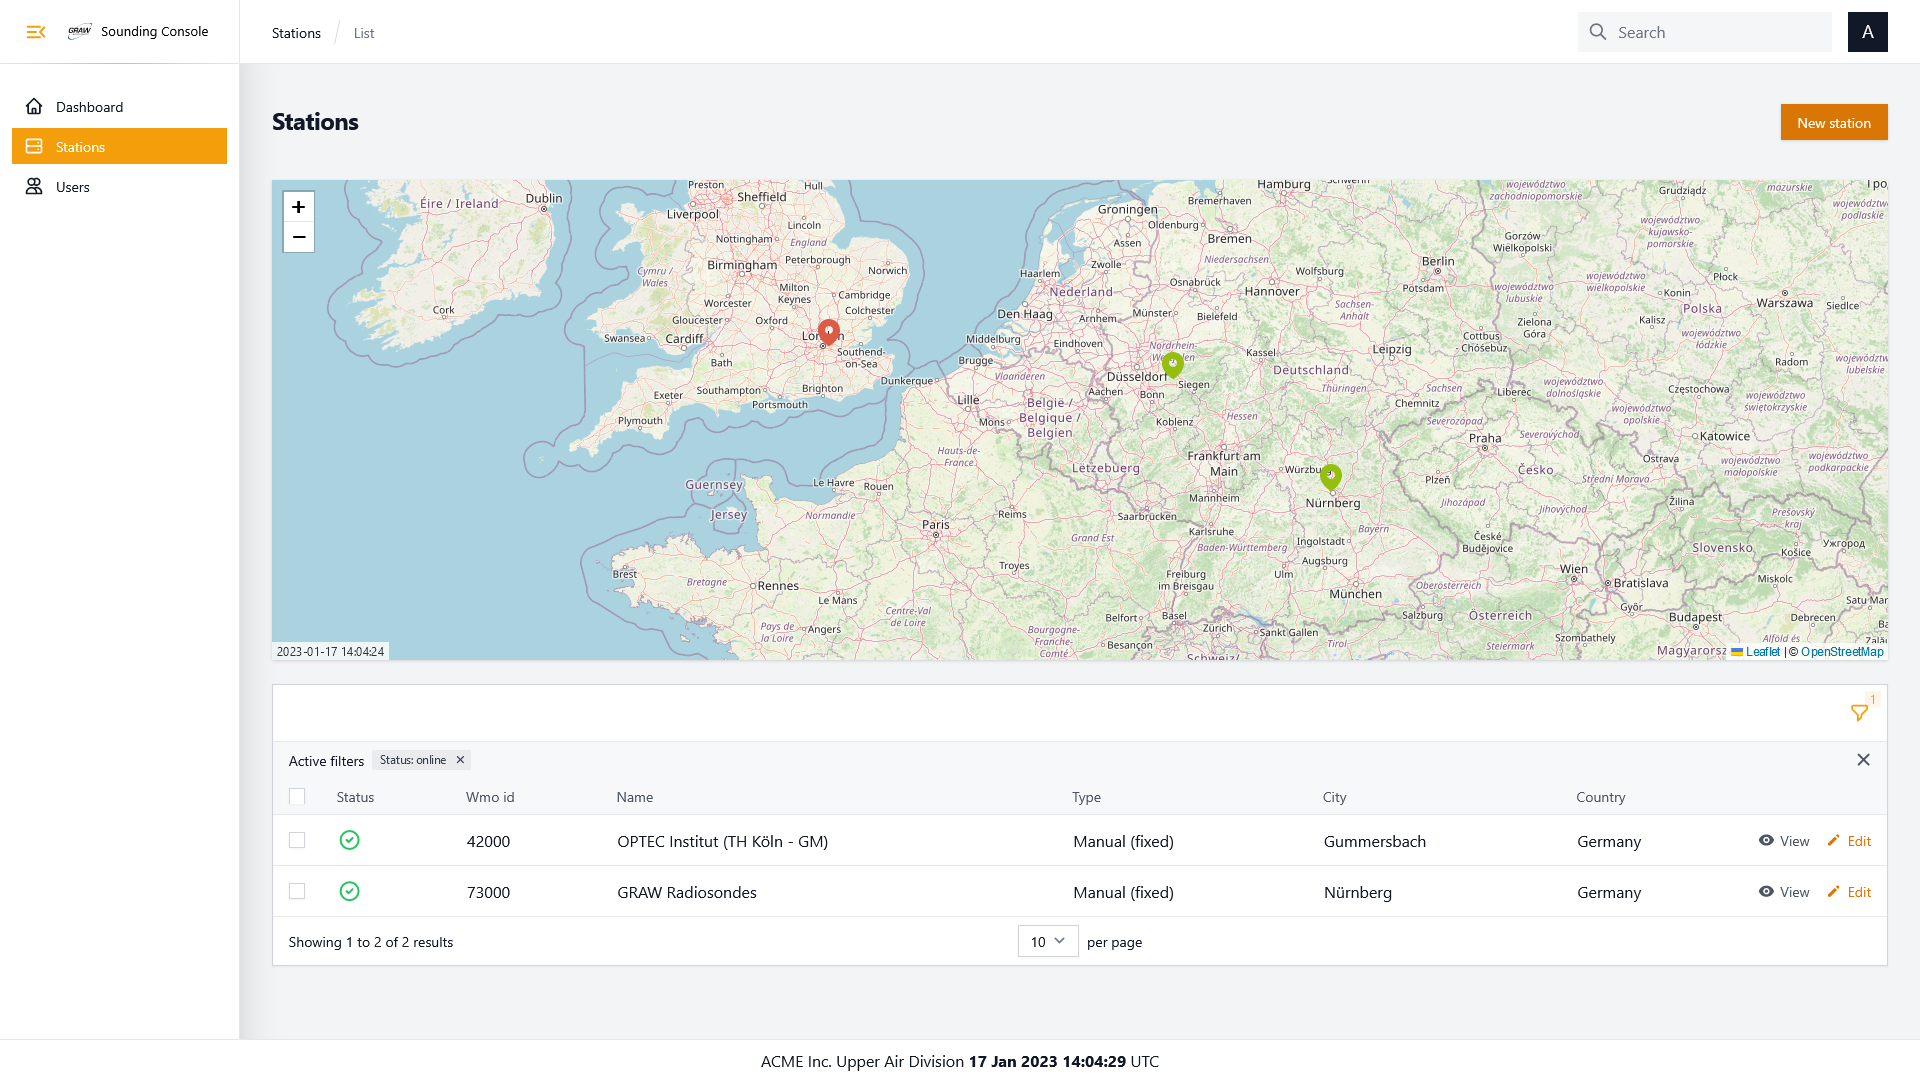
\includegraphics[scale=0.22]{assets/active_filter_filament}
\end{figure}

\begin{figure}[h!]
    \centering
    \caption{active filter nova}
    \label{fig:active_filter_nova}
    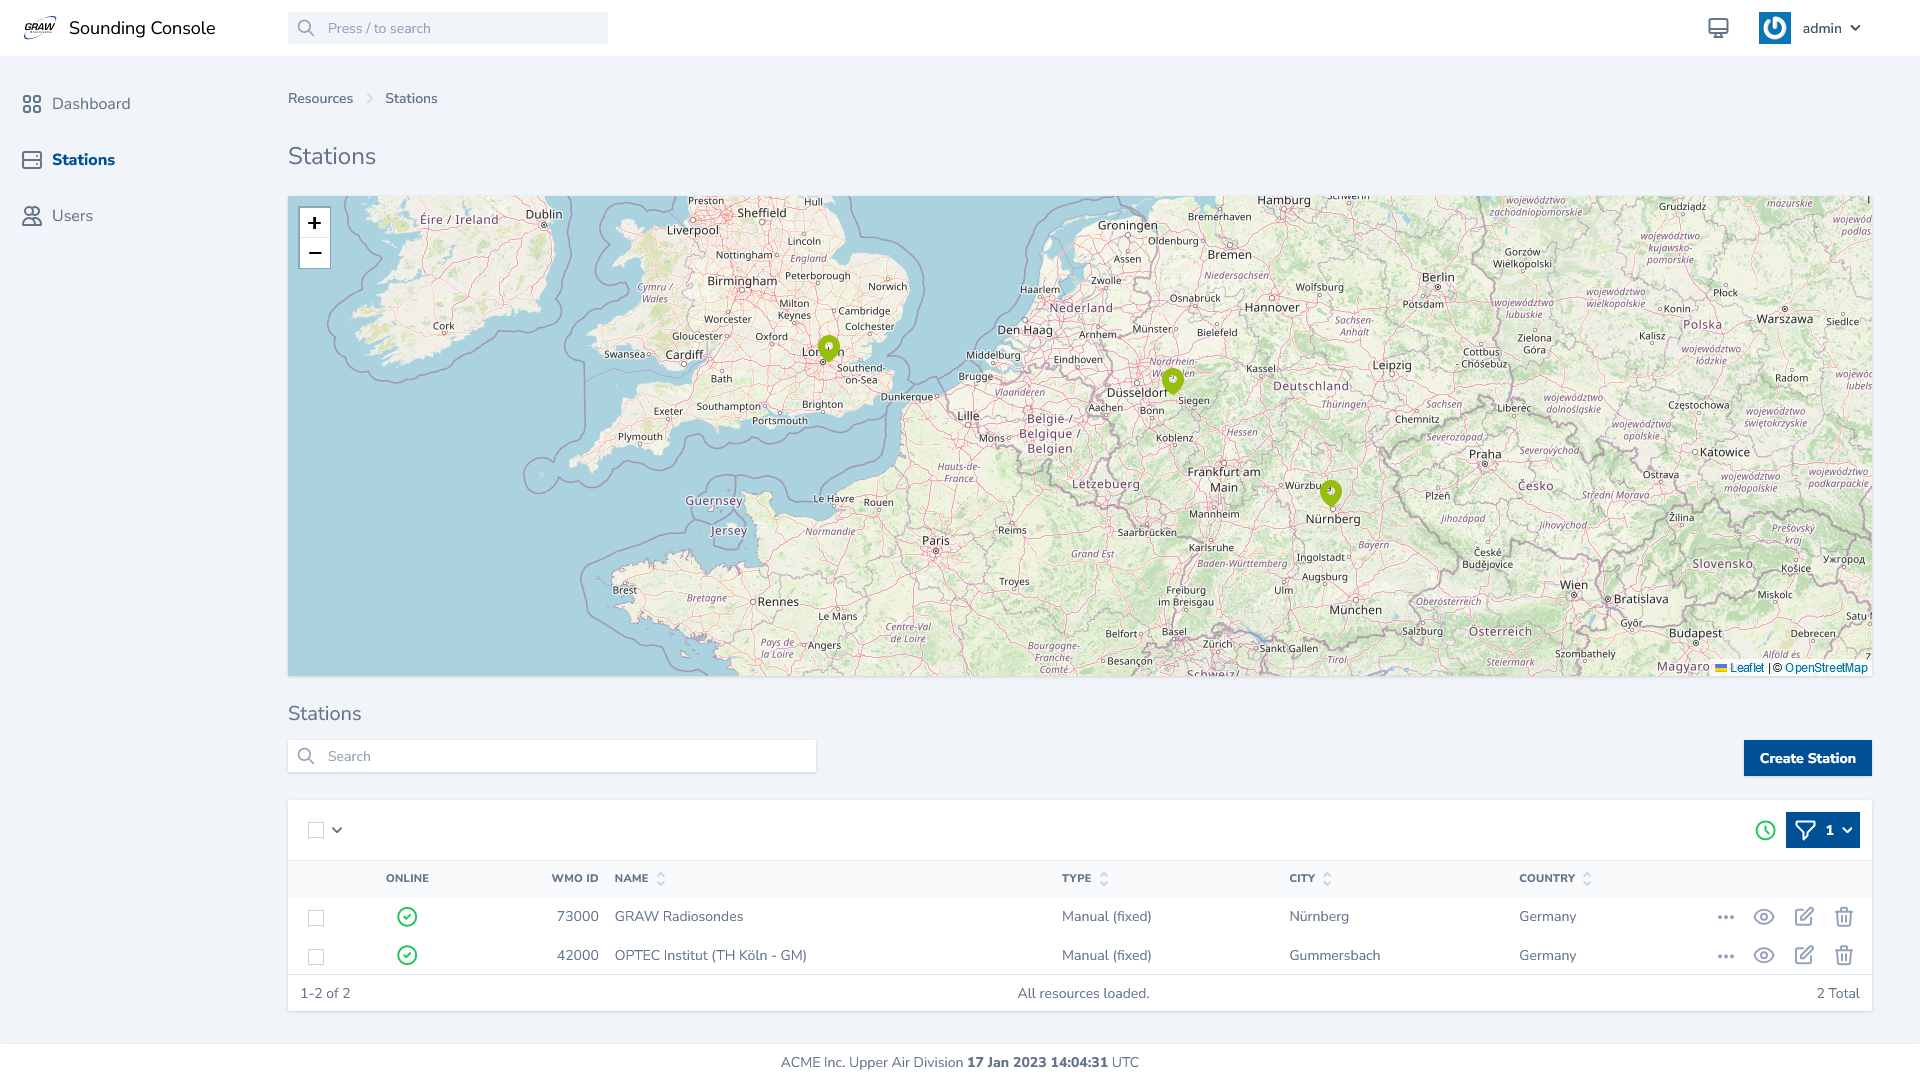
\includegraphics[scale=0.22]{assets/active_filter_nova}
\end{figure}

\newpage

\newlineparagraph{Flight View Anpassbarkeit}
Manche Ansichten benötigen weitreichende Anpassungen.
Hierzu zählt speziell der Blick auf einen vergangenen Flug.
Bei laufenden Flügen wird lediglich ein Dashboard mit aktuellen Werten und eine Karte angezeigt.
Beides passt sinnvoll oberhalb der restlichen Komponenten der Ressource, den Stammdatenfeldern und der Messwertetabelle.

Im Fall von vergangenen Flügen fällt das Dashboard weg, jedoch kommen ein Messdatendiagramm, eine Statistikübersicht und ein Skew-T-Diagramm hinzu.
Insgesamt sind das zu viele und zu große Komponenten, um diese direkt oberhalb auf der Seite zu platzieren.
Ein User müsste viel scrollen, um alles zu erfassen.
Dies wäre unübersichtlich und ineffizient.

Nova bietet kaum Möglichkeiten eine Ansicht anzupassen.
Daher war es die beste Variante, die Komponenten in Unterpunkte auszulagern (\ref{fig:finished_flight_nova}).
Nova unterstützt sogenannte Tools, welche eigenständige Seiten sind, auf denen individuelle Komponenten implementiert werden können.
Außerdem kann kontextabhängig das Menü angepasst werden.
Tests erster Nutzer zeigten allerdings, dass die entworfene Navigationsstruktur zu unübersichtlich ist.

Filament bietet gegenüber Nova weitaus mehr Möglichkeiten, eine Ansicht individuell anzupassen.
So kann bei der vorliegenden Herausforderung eine individuelle View für den Header angegeben werden.
Diese wird oberhalb aller anderen Komponenten auf der Ansichtsseite eines Fluges gerendert.
Innerhalb dieser individuellen View kann dann eine Tab View implementiert werden, die immer nur eine größere Komponente auf einmal anzeigt (\ref{fig:finished_flight_filament}).

Die Lösung mit filament überzeugt durch eine deutlich bessere User Experience.
Die komplizierte Navigationsstruktur im Menü entfällt komplett und alles findet direkt innerhalb der Flugansicht statt.
Längeres Scrollen entfällt und die Ansicht bleibt kompakt und übersichtlich.
Filament überzeugt durch die flexible und umfangreiche Anpassbarkeit.

\begin{figure}[h!]
    \centering
    \caption{finished flight filament}
    \label{fig:finished_flight_filament}
    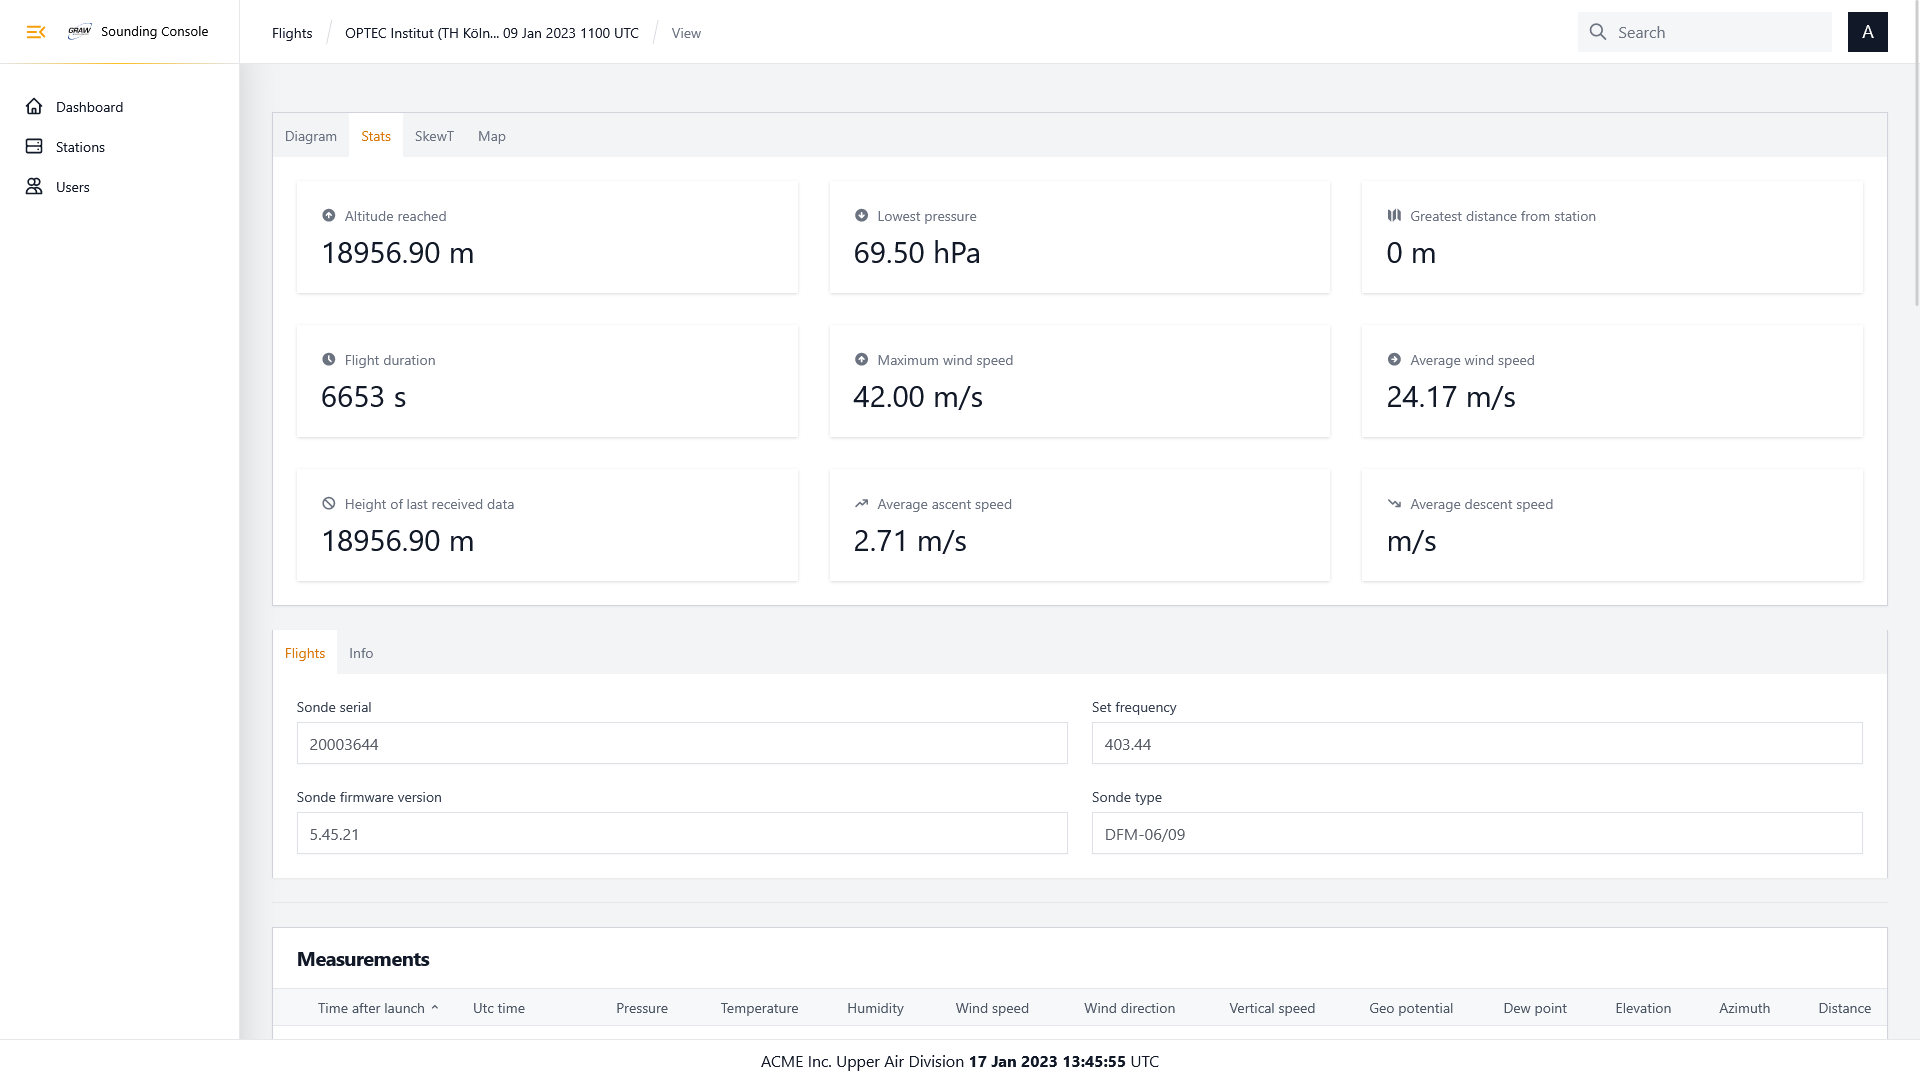
\includegraphics[scale=0.22]{assets/finished_flight_filament}
\end{figure}

\begin{figure}[h!]
    \centering
    \caption{finished flight nova}
    \label{fig:finished_flight_nova}
    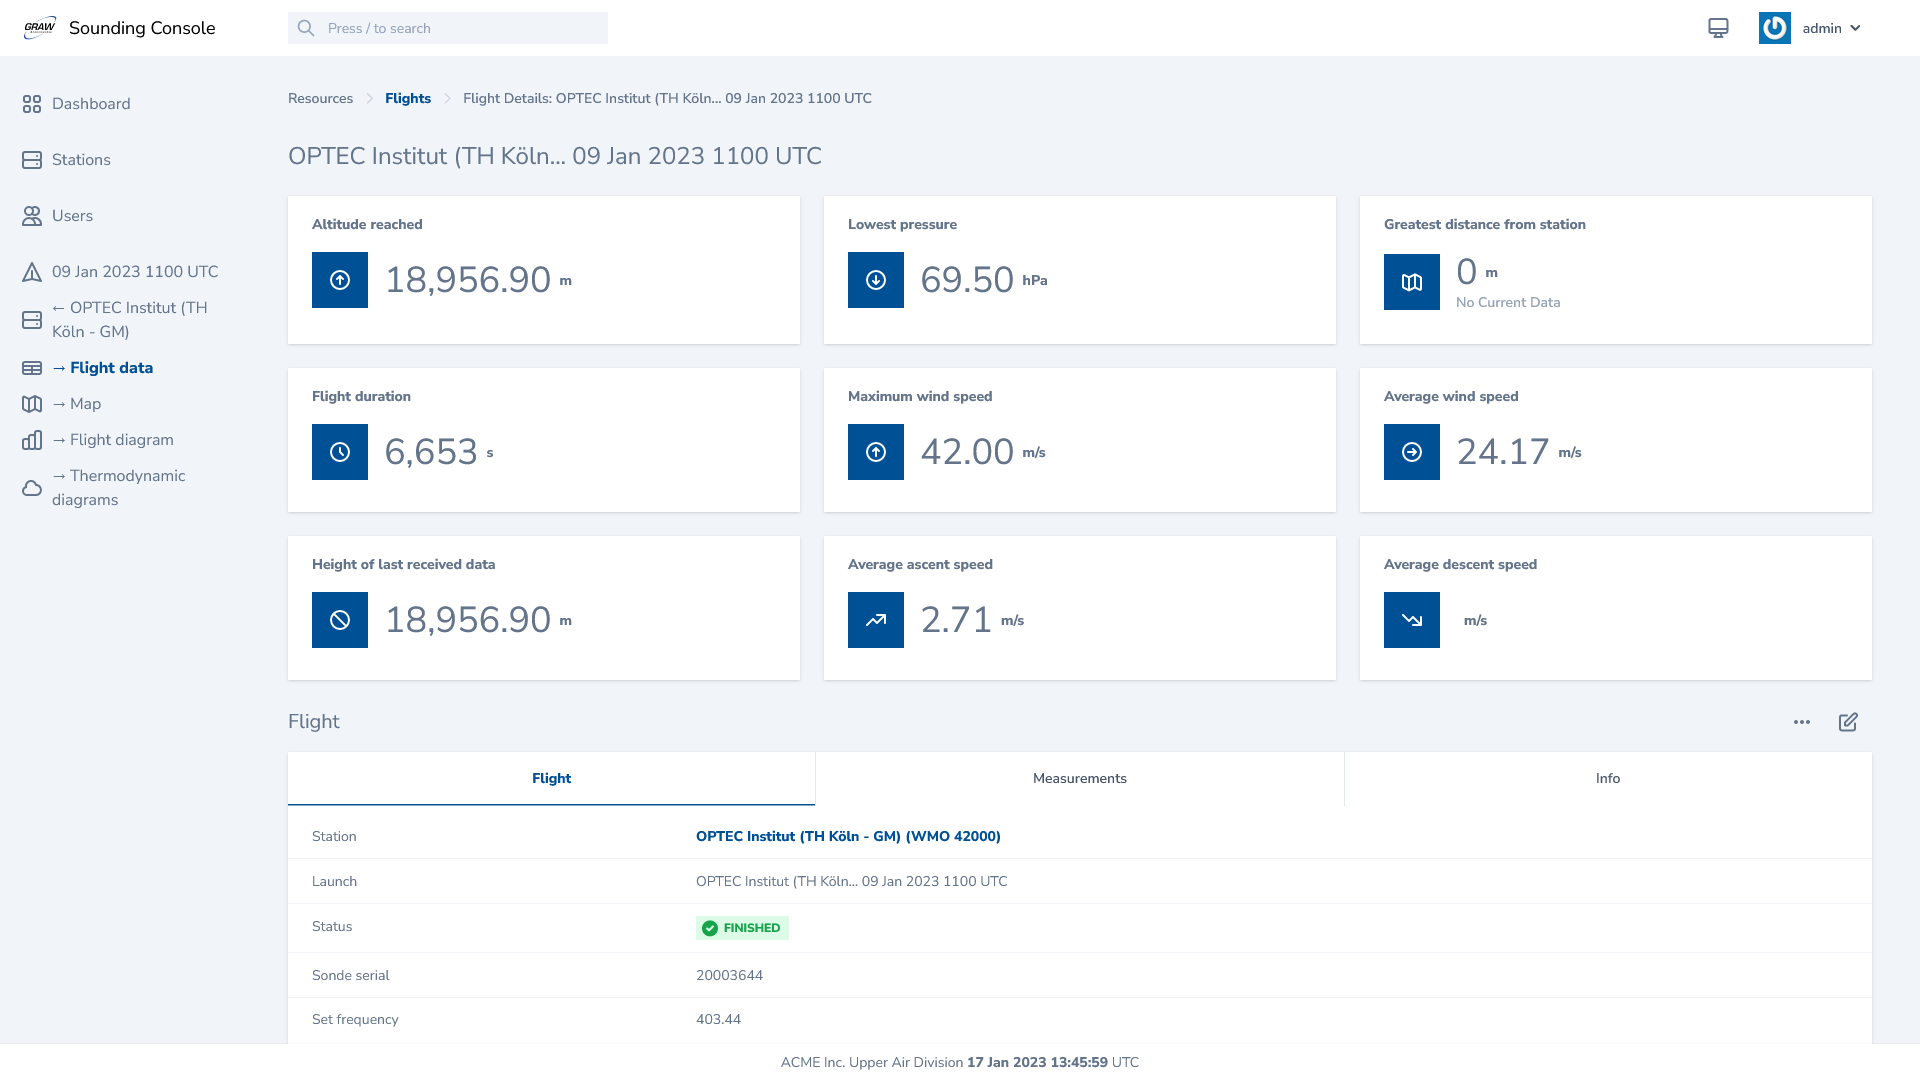
\includegraphics[scale=0.22]{assets/finished_flight_nova}
\end{figure}

\newpage

\newlineparagraph{Generelle Anpassbarkeit}
Filament punktet, durch eine generell flexiblere Anpassbarkeit.
Die Styles lassen sich besser anpassen.
Des Weiteren gibt es die Möglichkeit, an vielen Stellen individuelle Views einzuhängen.

\newlineparagraph{Ladeanimation der aktualisierenden Tabelle}
Filament zeigt keine Ladeanimation an, wenn die Tabelle neue Daten pollt.
Dadurch ist ein einfacher Vergleich der Werte möglich und die Seite springt nicht.
Die Seite springt nur, wenn neue Einträge hinzukommen.
Insgesamt ist die User Experience durch diese Animation bei filament wesentlich besser als bei Nova.

\newlineparagraph{Livewire Polling (Flight Dashboard Component)}
Filament basiert auf Livewire\cite{livewire} und somit können innerhalb einer individuellen Komponente auch Funktionen von Livewire genutzt werden.
So gibt es einen eingebauten Polling Mechanismus.
Man fügt lediglich ein Attribut zu einem HTMl Objekt hinzu und Livewire ruft dieses in einem definierbaren Intervall erneut vom Server ab.

So wurde die Implementierung des Dashboards eines laufenden Fluges vereinfacht.
Die Api und manuelles Polling mit anschließendem Austausch der Datenbasis, sodass Vue.js den Inhalt dann reaktiv updaten kann, wird nicht mehr benötigt.
Es muss nur innerhalb der Blade Komponente mit serverseitigem Code das Dashboard generiert werden und Livewire übernimmt den Rest vollautomatisch.

\newlineparagraph{Styling von Custom Components}
Nova unterstützt explizit die Verwendung der Blade Components.
So können fertige Funktionen und einheitliche Stile wiederverwendet werden.
Bei der Sounding Console werden beispielsweise Widgets als fertige Komponente geladen.

\newpage

\newlineparagraph{Infinite Loading Tables}
Filament schafft es, eine benutzbare UI mit mehreren tausenden geladenen und angezeigten Zeilen in einer Tabelle zu rendern.
Damit ist im Gegensatz zu Nova kein Infinite Load/Scroll Pattern notwendig.

Außerdem zeigt filament standardmäßig auch eine \enquote{All} Option für die Pagination an.
Dadurch kann eine zu nativen Anwendungen vergleichbare UI erstellt werden, in welcher der User durch die vollständige Tabelle scrollen kann.

\newlineparagraph{Tabellensortierung}
Ist bei filament eine Spalte als sortierbar definiert, kann für eine Ansicht ebenfalls eine Standardsortierung angegeben werden.
Dabei ist sowohl die Angabe der Spalte möglich, als auch die Sortierrichtung.
Das Problem mit Nova wird, durch diese implementierte Lösung, vollständig gelöst.

\subsubsection{Negative Erfahrungen}
Trotz aller positiven Erfahrungen gab es auch eine Hürde mit filament, welche im Folgenden erläutert ist.
Diese konnte allerdings überwunden werden, es musste lediglich auf ein neues Konzept umgestellt werden.

\newlineparagraph{Livewire Polling (Map Component)}
Das Livewire Polling Konzept ist nicht immer von Vorteil.
Bei einfachen Komponenten ist es sinnvoll, bei komplexeren Komponenten wie zum Beispiel der Karte, ist es problematisch.
Mit Nova war die Umsetzung etwas einfacher, da individuelle Nova Komponenten bereits eine geschützte HTTP Api vorbereiten, über die Updates regelmäßig abgerufen werden können.
Das Polling der gesamten Komponente ist mit filament keine Option, dennoch müssen Veränderungen erkannt und automatisch angezeigt werden.
Durch das Attribut \enquote{wire:ignore} können allerdings einzelne Bestandteile ausgenommen werden.
So wird die Karte und das dazugehörige Script nicht erneut geladen, sondern nur ein Teil, welcher bei einem Update ein Event aussendet, auf welches die Karte dann reagiert.

\newpage

\subsubsection{Implizit versus explizit}
Die prototypischen Erfahrung entsprechen denen, über die andere Entwickler\cite{reddit-laravel-nova-vs-filament} bereits berichteten.
Nova arbeitet impliziter als filament:
Felder werden an einer Stelle definiert, diese gelten dann sowohl für das Formular, als auch für die Tabelle.
Bei filament wird ein Feld mindestens an zwei Stellen definiert.

Grundsätzlich erwartet filament, dass für jede eigene Tabelle die Spalten erneut explizit definiert werden.
Dies lässt sich jedoch umgehen, indem die Tabelle aus der Ressource referenziert wird.

Die unterschiedlichen Ansätze haben ihre Vor- und Nachteile.
Der implizite Ansatz bei Nova ist schneller, insbesondere am Anfang.
Filaments explizite Definitionen benötigen initial mehr Zeit, überzeugen aber am Ende durch eine bessere und einfachere Anpassbarkeit.
Zudem ist es durchaus sinnvoll, explizit zu formulieren, wie die Felder im Formular und wie sie in Tabellen dargestellt werden sollen.
So wird verhindert, dass unerwartete Fälle eintreten, da mindestens einmal während der Entwicklung durchdacht werden muss, wie jeder Fall explizit definiert wird.


    \section{Reflektion}

    \section{Fazit und Ausblick}

\subsection{Fazit}
tbd

\subsection{Ausblick}
tbd


    \appendix

\newpage


\section{Quellenverzeichnis}
\bibliographystyle{plain}
\printbibliography


\section{Abbildungsverzeichnis}
\listoffigures

\newpage


\section{Anhang}

\subsection{Eigenständigkeitserklärung}

\textbf{Eidesstattliche Erklärung}

Ich versichere, die von mir vorgelegte Arbeit selbständig verfasst zu haben.

Alle Stellen, die wörtlich oder sinngemäß aus veröffentlichten oder nicht veröffentlichten Arbeiten anderer entnommen sind, habe ich als entnommen kenntlich gemacht.
Sämtliche Quellen und Hilfsmittel, die ich für die Arbeit benutzt habe, sind angegeben.

Die Arbeit hat mit gleichem Inhalt bzw.\ in wesentlichen Teilen noch keiner anderen Prüfungsbehörde vorgelegen.


\includegraphics[scale=0.5]{assets/signature}\\
Gummersbach, den \today

\end{document}
